\subsection{Unregelmäßigkeiten in der Klassifikation des Portals "`\gls{bapvs}"'}
    Die Klassifikation des Lehrgebietes \gls{bapvs}
    weist ebenfalls einige Unregelmäßigkeiten auf,
    die dieses Kapitel beschreibt.

    \paragraph{Doppelt klassifizierte Mitarbeiter}
    Drei Mitarbeiter des Portals wurden doppelt klassifiziert.
    Der Grund ist eine abweichende HTML-Struktur bei diesen Mitarbeitern,
    die in Listing \ref{listing:findingsTeachersBaPVSHtmlSource} zu sehen ist.

    \lstinputlisting[
        label=listing:findingsTeachersBaPVSHtmlSource,
        caption=Abweichende HTML-Struktur eines Mitarbeiters im Portal BaPVS,
        style=html
    ]{../resources/findings/case-study-1/bapvs/teacher.html}

    Im Vergleich zur erwarteten Struktur\footnote{vgl. Listing \ref{listing:findingsTeachersHtmlSource}} wiederholt sich
    das \texttt{div}-Element mit der Klasse \texttt{grid},
    weshalb der verwendete Selektor \texttt{section\#content div.grid}
    betroffene Mitarbeiter doppelt erfasst.
    Im Fall von zwei Mitarbeitern kann das System bei der zweiten Klassifizierung
    (beim inneren \texttt{div}-Element) kein Bild finden,
    weshalb sie von der ersten abweicht und ein zweiter \texttt{Teacher}-Knoten angelegt wird.
    Diese teilen sich aber die restlichen Informationen,
    also Name, Lehrgebiet und Kontaktinformationen.
    Im dritten Fall besitzt der Mitarbeiter kein Bild,
    weshalb der \texttt{Teacher}-Knoten vollständig wiederverwendet werden kann.

    \paragraph{Mitarbeiter ohne Lehrgebiet}
    Das Lehrgebiet eines einzelnen Mitarbeiters wurde vom System nicht erfasst.
    Anders als beim Lehrgebiet \gls{babw} ist der Grund allerdings,
    dass vor dem Lehrgebiet der Text "`Auskunft erteilt auch:"' platziert ist.
    Der Selektor \texttt{div.team-member-des > p > a:first-child} findet
    kein Lehrgebiet, weil er nach einem \texttt{a}-Element sucht,
    welches das erste Kindelement seines Vaterelementes ist.
    Eine naheliegende Lösung ist die Änderung des Selektors,
    sodass er mit \texttt{a:first-of-type} endet.
    Bei der Erstellung des {\classificationModel}s,
    was auf Basis des Portals \gls{babw} geschah,
    wurde sich allerdings bewusst gegen diese Variante entschieden.
    Bei dem Mitarbeiter im \gls{babw}, für den kein Lehrgebiet erfasst
    wurde\footnote{vgl. Kapitel \ref{section:findingsTeachersAbnormalitiesBabw}},
    hätte dieser Selektor nämlich dazu geführt,
    dass seine E-Mail-Adresse als Lehrgebiet erkannt wird.

    \paragraph{Falscher Text als Name klassifiziert}
    Der Name eines gewissen Mitarbeiters ist laut Klassifikation
    "`Auskunft erteilt auch:"'.
    Der Grund ist, dass dieser Text in einem \texttt{strong}-Element steht,
    welches vor dem Namen auftaucht.
    Das System hat in diesem Fall erwartungskonform nur den ersten
    Treffer für das skalare Feature klassifiziert.
        
    \paragraph{28 Mitarbeiter ohne Telefonnummer}
    Einige Kontakte besitzen in der Klassifikation keine Telefonnummer.
    Bei neun ist auch auf der Webseite keine zu finden.
    Bei den restlichen ist der Nummer nicht "`Tel.: "'
    sondern "`Telefon: "' oder "`Tel:"' vorangestellt.
    Der Selektor hat die Telefonnummern deshalb nicht erkannt.
    
    \paragraph{56 Mitarbeiter ohne Namen}
    Des Weiteren wurde für eine Vielzahl der Mitarbeiter kein Name erkannt,
    da sie weder in einem \texttt{strong} noch einem \texttt{b} Element stehen.
    Stattdessen befinden sie sich wie die Telefonnummer als reiner Text im Element
    oder in einem \texttt{a}-Element.

    \paragraph{Inkorrekte Telefonnummern}
    Die Klassifikation enthält einige Telefonnummern,
    die neben der eigentlichen Nummer auch weitere Informationen enthalten.
    Ein Beispiel ist "`02331/987-4315 email: Lisa.Schaefer Sprechstunde: nach Vereinbarung via e-mail"'.
    Die Telefonnummer wird über einen {\xpathSelector} erfasst,
    der auf dem Seitenquelltext ausgeführt wird.
    Anders als beim Portal \gls{babw} existieren in \gls{bapvs} Mitarbeiter,
    bei denen die Telefonnummer weder die letzte Angabe ist
    noch durch einen physischen Zeilenumbruch im Quelltext gefolgt wird.
    Der Selektor der Telefonnummer erkennt sie deshalb
    nicht\footnote{vgl. Kapitel \ref{section:findingsTeachersClassificationModel}}.

    \paragraph{Unterschiede im konzeptionellen Modell der Seite}
    Im Vergleich zur klassifizierten Seite des Portals \gls{babw}
    sind auch zwei Unterschiede im konzeptionellen Modell der Seite deutlich geworden.
    Der Name eines Mitarbeiters ist in einigen Fällen
    auch ein Link auf eine Detailseite.
    Außerdem besitzen einige Mitarbeiter Sprechzeiten.

    \paragraph{Falsch annotierte Telefonnummern}
    \textbf{DAS IST EIN BUG -- SOLL DAS DRIN BLEIBEN? WIRD DAS IN DER DISCUSSION NOCHMAL AUFGEGRIFFEN}
    Bei der Betrachtung der Annotationen des Portals \gls{babw}
    ist bereits aufgefallen, dass sie für Telefonnummern
    mehrmals verschoben sind.
    Dies ist im Fall des Portals \gls{bapvs} ebenfalls zu beobachten,
    allerdings in einem deutlicheren Ausmaß,
    wie Abbildung \ref{image:findingTeachersBaPVSWrongPhone} zeigt.

    \begin{figure}[htb]
        \centering
        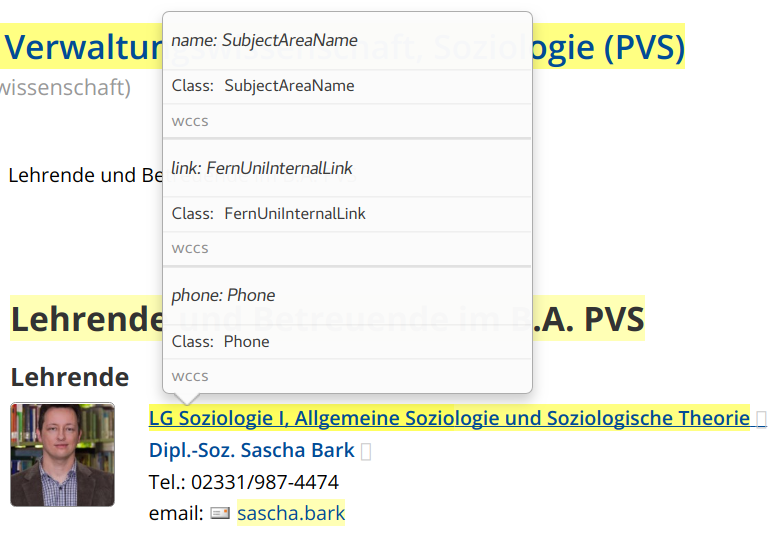
\includegraphics[scale=\screenshotScaleFactor]{../resources/findings/case-study-1/bapvs/annotations/triple-annotation.png}
        \caption{Verschobene Annotation einer Telefonnummer im \gls{bapvs}}
        \label{image:findingTeachersBaPVSWrongPhone}
    \end{figure}

    Bei der Bestimmung des eindeutigen Selektors,
    wird die Position des klassifizierten Textes in der Eigenschaft
    \texttt{innerText} als Versatz im Startelement
    verwendet\footnote{vgl. Kapitel \ref{section:solutionDetailsClassificationServiceClassification}}.
    In den betroffenen Fällen befindet sich zwischen der Telefonnummer
    und der E-Mail-Adresse nur ein \texttt{br}-Element,
    aber kein physischer Zeilenumbruch im
    Seitenquelltext\footnote{vgl. Listing \ref{listing:findingsTeachersHtmlSource}}.
    Die Telefonnummer, die über einen {\xpathSelector} ermittelt wird,
    enthält deshalb zu viele Informationen (siehe oben),
    die wiederum nur durch ein Leerzeichen, aber nicht durch einen Zeilenumbruch getrennt sind.
    In \texttt{innerText} wird das \texttt{br}-Element aber zu einem Umbruch,
    weshalb der klassifizierte Text in dieser Eigenschaft nicht gefunden wird.
    Als Versatz wird deshalb $-1$ gespeichert.
    Annotator setzt die Annotation deshalb an den Anfang des umschließenden Elementes.
